\documentclass[12pt]{article}
\usepackage{amsmath, fullpage}
\usepackage{graphicx}

\begin{document}

\title{Efectos de la red}
\author{Jesus H. Abundis}
%\date{\vspace{-5ex}}
\maketitle
\thispagestyle{empty}

En la programación tradicional de un único equipo, 
podemos construir aplicaciones con un alto grado de concurrencia debido a los múltiples núcleos de cómputo con que contamos en los sistemas modernos.
La manera en que aprovechamos estos recursos es a través de hilos (threads).
La comunicación entre hilos en tales programas es normalmente implícita debido a que los hilos comparten un único espacio de direcciones común debido a que pertenecen al mismo proceso.
Más aún, 
ya que utilizamos un sólo equipo, 
todos los hilos pueden acceder a la misma memoria física compartida.
El principal problema que tenemos es manipular el acceso concurrente y evitar condiciones de carrera, 
lo cual atendemos mediante la sincronización de los hilos,
mediante un seguro en los hilos,
o utilizando hardware para operaciones atómicas 
(La habilidad de un procesador o GPU para llevar acabo operaciones de lectura, escritura, o modificación de la memoria como una unidad única, indivisible e ininterrumpida, previniendo la corrupción de datos por parte de hilos concurrentes).

\begin{figure}[h]
   \centering
   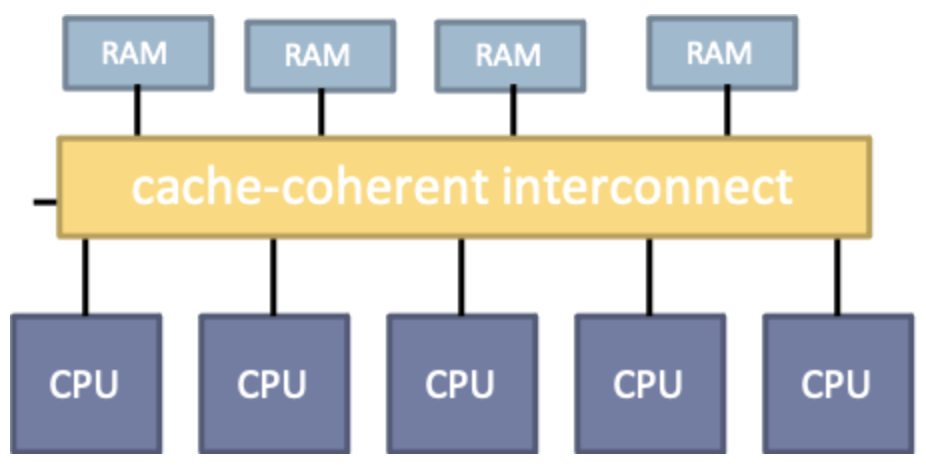
\includegraphics[scale=0.5]{single_pc_arquitecture.png}
\end{figure}

Los sistemas distribuidos son fundamentalmente distintos de los computadores únicos debido a su falta de memoria compartida.
Debido a que en la mayoría de escenarios deseamos utilizar multiples equipos de manera coordinada y colaborar en un problema compartido,
debemos llevar acabo una comunicación explícita.
En esencia, debemos mandar mensajes a través de la red en todo lugar dónde un programa concurrente en una única computadora sería capaz de tener acceso a su memoria compartida.

\begin{figure}[h]
   \centering
   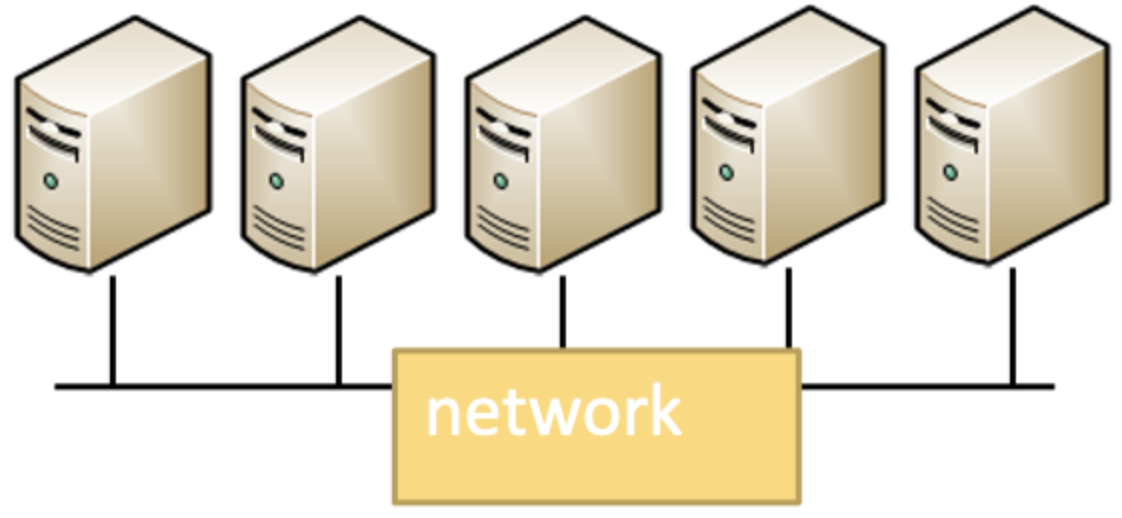
\includegraphics[scale=0.5]{red_computadoras.png}
\end{figure}


Las redes tradicionales tienen distintas desventajas en comparación con la comunicación implícita en un computador. 
Consideremos la siguiente abstracción de una red de comunicación:

\begin{figure}[h]
   \centering
   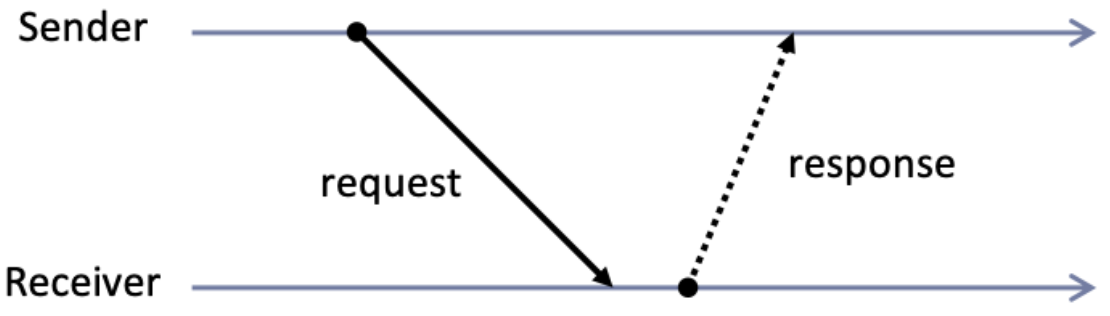
\includegraphics[scale=0.5]{red_comunicacion.png}
\end{figure}

En esta imagen tenemos un emisor (sender) enviando un request al receptor (receiver).
El receptor procesa el request y envía de vuelta una respuesta. 
Si no hay problemas en la red esto es una comunicación exitosa.
Sin embargo, bajo ciertas condiciones, 
este mensaje puede perderse o experimentar largos retrasos.
Debido a esto,
el receptor puede optar por enviar inmediatamente un mensaje de recibido para el conocimiento del emisor.
Esta mensaje, siendo un mensaje, también puede perderse o retrasarse.
Lo mismo sucede con el mensaje de respuesta.

No importa como diseñemos el protocolo, debemos lidiar con la asincronía de la red física y la potencial pérdida de mensajes debida,
por ejemplo,
al llenado del queue de los routers,
posteriormente a los cual los mensajes son rechazados.
Más aún, 
ya que ambas computadoras son independientes la una de la otra,
también pueden fallar de manera independiente, 
o bien la red entre ellos podría sufrir una caída.
En esencia, 
existe una incertidumbre sin límite en el tiempo en el envío de mensajes en una red asíncrona debido a que no podemos distinguir entre un mensaje perdido o uno retrasado.

La solución práctica a este problema es implementar un límite en el tiempo a partir del cual declararemos un mensaje retrasado como perdido.
Esto crea un problema cuando la operación emitida por el mensaje no es idempotente  ya que, en este caso, debemos evitar ejecutarla más de una vez.
En protocolos reales, 
podríamos emitir IDs en los mensajes para filtrar duplicados.

A pesar de todos los esfuerzos,
existen desafíos adicionales en una arquitectura distribuida.
EN comparación con la memoria compartida,
la memoria distribuida puede contener múltiples replicas de la misma información,
tal que podemos tener un problema de consistencia 
(datos únicos y válidos)
debido a que las actualizaciones se propagan a través de los mensajes y los mensajes pueden perderse.

A partir de estas consideraciones, 
podemos concluir que tener un sistema distribuído nunca es el objetivo final sino una alternatica que tomamos para lograr propiedades que son difíciles o imposibles con un sólo equipo.
Tenemos como ejemplos la escalabilidad para problemas muy grandes,
la resistencia a fallos a través de la redundancia,
para lo cual necesitamos múltiples instancias.

Por naturaleza, 
los sistemas centralizados tienen modelos de falla más simple debido a que tienden a fallar completamente o funcionar,
tienen una latencia menor debido a la falta de una red y son más fáciles de programar debido a su memoria compartida.
En resumen, nunca quieres un sistema distribuido pero en frecuentemente lo necesitas.


\end{document}
